\section{BP5-QD}
\subsection{SBP-SAT formulations for BP5-QD}
For this 3D problem, we use SBP-SAT methods similar to \cite{ALMQUIST2021109842} to formulate our linear system.
To solve the linear elasticity in 3D, we need to solve for the displacements in $x$, $y$, and $z$ directions for each point.
We denote the displacement vector as $\boldsymbol{u} = [u_1, u_2, u_3]$.
To turn the tensor formulation from \cite{ALMQUIST2021109842} into a matrix formulation for iterative solvers,  we first stack the displacements for a point in $x$, $y$, $z$ directions, and then for all points in $x$, $y$, and $z$ directions.
We label the faces for 3D simulation in the following order as shown in Figure \ref{fig:3d_problem}

\begin{figure}
    \centering
    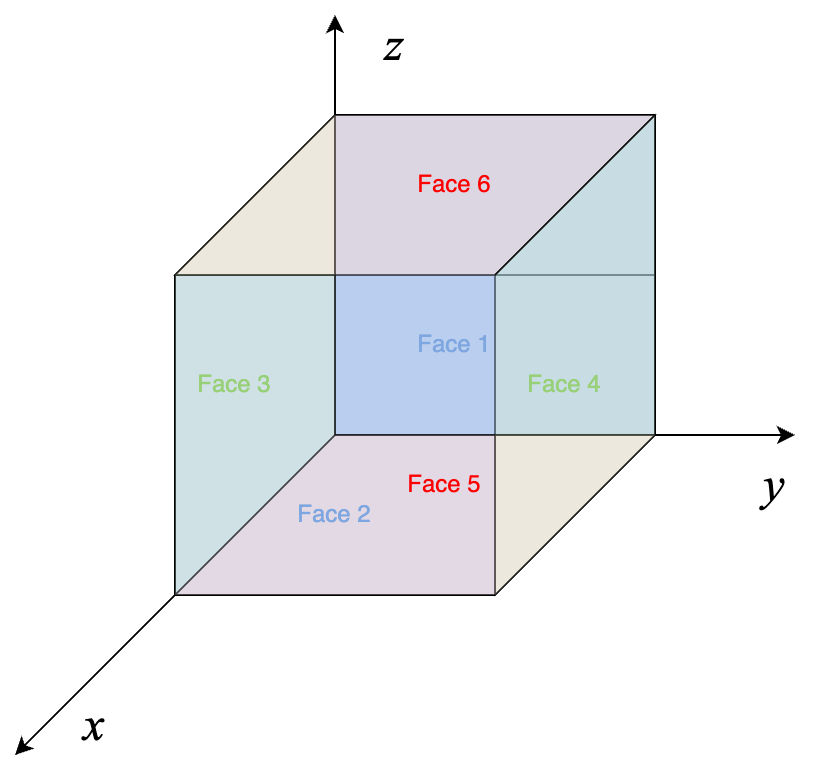
\includegraphics[width=\linewidth]{figures/3D_problem.png}
    \caption{We set up the 3D coordinate and denote faces 1 to 6 using different colors. Face 1 and Face 2 are perpendicular to the x-axis denoted using blue color. Face 3 and Face 4 are perpendicular to the y-axis denoted using green color. Face 5 and Face 6 are perpendicular to the z-axis denoted using red color. We impose Dirichlet boundary conditions on Face 1 and Face 2. For Face 3 to Face 6, we impose traction-free (Neumann) condition.} 
    \label{fig:3d_problem}
\end{figure}

The first step is to derive values for $\sigma$ tensor in 3D.

\begin{align}
    \sigma_{11} = K\epsilon_{kk} + 2\mu (\epsilon_{11} - \frac{1}{3}\epsilon_{kk}) &= (K - \frac{2}{3}\mu)( \frac{\partial u_1}{\partial x_1} + \frac{\partial u_2}{\partial x_2} + \frac{\partial u_3}{\partial x_3}) + 2\mu \frac{\partial u_1}{\partial x_1} \\
    \sigma_{12} = 2\mu \epsilon_{12} &= \mu(\frac{\partial u_1}{\partial x_2} + \frac{\partial u_2}{\partial x_1}) \\
    \sigma_{13} = 2\mu \epsilon_{13} &= \mu(\frac{\partial u_1}{\partial x_3} + \frac{\partial u_3}{\partial x_1}) \\
    \sigma_{21} = 2\mu \epsilon_{21} &= \mu(\frac{\partial u_2}{\partial x_1} + \frac{\partial u_1}{\partial x_2}) \\
    \sigma_{22} = K\epsilon_{kk} + 2\mu (\epsilon_{22} - \frac{1}{3}\epsilon_{kk}) &= (K - \frac{2}{3}\mu)( \frac{\partial u_1}{\partial x_1} + \frac{\partial u_2}{\partial x_2} + \frac{\partial u_3}{\partial x_3}) + 2\mu \frac{\partial u_2}{\partial x_2} \\
    \sigma_{23} = 2\mu \epsilon_{13} &= \mu(\frac{\partial u_2}{\partial x_3} + \frac{\partial u_3}{\partial x_2}) \\
    \sigma_{31} = 2\mu \epsilon_{31} &= \mu(\frac{\partial u_3}{\partial x_1} + \frac{\partial u_1}{\partial x_3}) \\
    \sigma_{32} = 2\mu \epsilon_{32} &= \mu(\frac{\partial u_3}{\partial x_2} + \frac{\partial u_2}{\partial x_3}) \\
    \sigma_{33} = K\epsilon_{kk} + 2\mu (\epsilon_{33} - \frac{1}{3}\epsilon_{kk}) &= (K - \frac{2}{3}\mu)( \frac{\partial u_1}{\partial x_1} + \frac{\partial u_2}{\partial x_2} + \frac{\partial u_3}{\partial x_3}) + 2\mu \frac{\partial u_3}{\partial x_3}
    \label{eqn:sigma-tensor}
\end{align}


Here, we also use $1,2,3$ to denote the components of $\sigma$ in $x,y,z$ directions to simplify the notation.
Then we can rewrite governing equations in terms of the $x,y,z$ components.

\begin{align}
    \rho \frac{\partial^2{u_1}}{\partial{t^2}} &= \frac{\partial \sigma_{11}}{\partial x_1} + \frac{\partial \sigma_{12}}{\partial x_{2}} + \frac{\partial \sigma_{13}}{\partial x_{3}} \nonumber \\
    &= (K - \frac{2}{3}\mu)( \frac{\partial^2 u_1}{\partial x_1^2} + \frac{\partial^2 u_2}{\partial x_1 \partial x_2} + \frac{\partial^2 u_3}{\partial x_1 \partial x_3}) + 2\mu \frac{\partial^2u_1}{\partial x_1^2} \nonumber \\
        & + \mu(\frac{\partial^2 u_1}{\partial x_2^2} + \frac{\partial^2u_2}{\partial x_2 \partial x_1})
        + \mu(\frac{\partial^2 u_1}{\partial x_3^2} + \frac{\partial^2u_3}{\partial x_3 \partial x_1}) \\
    \rho \frac{\partial^2{u_2}}{\partial{t^2}} &= \frac{\partial \sigma_{21}}{\partial x_1} + \frac{\partial \sigma_{22}}{\partial x_{2}} + \frac{\partial \sigma_{23}}{\partial x_{3}} \nonumber \\
    &= \mu(\frac{\partial^2u_2}{\partial x_1^2} + \frac{\partial^2 u_1}{\partial x_1 \partial x_2})
    + (K - \frac{2}{3}\mu)( \frac{\partial^2 u_1}{\partial x_2 \partial x_1} + \frac{\partial^2 u_2}{\partial x_2^2} + \frac{\partial^2 u_3}{\partial x_2 \partial x_3}) \nonumber \\
    &+ 2\mu \frac{\partial^2u_2}{\partial x_2^2} 
    + \mu(\frac{\partial^2u_2}{\partial x_3^2} + \frac{\partial^2 u_3}{\partial x_3 \partial x_2}) \\
    \rho \frac{\partial^2{u_3}}{\partial{t^2}} & = \frac{\partial \sigma_{31}}{\partial x_1} + \frac{\partial \sigma_{32}}{\partial x_{2}} + \frac{\partial \sigma_{33}}{\partial x_{3}} \nonumber \\
    &= \mu(\frac{\partial^2u_3}{\partial x_1^2} + \frac{\partial^2 u_1}{\partial x_1 \partial x_3}) \nonumber
    + \mu(\frac{\partial^2 u_3}{\partial x_2^2} + \frac{\partial^2u_2}{\partial x_2 \partial x_3}) \\
    & + (K - \frac{2}{3}\mu)( \frac{\partial^2 u_1}{\partial x_3 \partial x_1}   + \frac{\partial^2 u_2}{\partial x_3 \partial x_2} + \frac{\partial^2 u_3}{\partial x_3^2}) + 2\mu \frac{\partial^2u_3}{\partial x_3^2} 
    \label{eqn:components}
\end{align}

We can use them to impose the SAT terms for displacements in $x, y, z$ directions using formulations from \cite{ALMQUIST2021109842}.
For Neuman boundary conditions, we have
\begin{align}
    SAT_1 = &-H^{-1} [e_3 H_3 (e_3^T [T_{11}^3 u_1 + T_{12}^3 u_2 + T_{13}^3 u_3] - g_1^3)] \nonumber \\
&- H^{-1} [e_4 H_4 (e_4^T [T_{11}^4 u_1 + T_{12}^4 u_2 + T_{13}^4 u_3] - g_1^4)] \nonumber \\
&- H^{-1} [e_5 H_5 (e_5^T [T_{11}^5 u_1 + T_{12}^5 u_2 + T_{13}^5 u_3] - g_1^5)] \nonumber \\
&- H^{-1} [e_6 H_6 (e_6^T [T_{11}^6 u_1 + T_{12}^6 u_2 + T_{13}^6 u_3] - g_1^6)] \\
SAT_2 = &-H^{-1} [e_3 H_3 (e_3^T [T_{21}^3 u_1 + T_{22}^3 u_2 + T_{23}^3 u_3] - g_2^3)] \nonumber \\
& - H^{-1} [e_4 H_4 (e_4^T [T_{21}^4 u_1 + T_{22}^4 u_2 + T_{23}^4 u_3] - g_2^4)] \nonumber \\
& - H^{-1} [e_5 H_5 (e_5^T [T_{21}^5 u_1 + T_{22}^5 u_2 + T_{23}^5 u_3] - g_2^5)] \nonumber \\
& - H^{-1} [e_6 H_6 (e_6^T [T_{21}^6 u_1 + T_{22}^6 u_2 + T_{23}^6 u_3] - g_2^6)] \\
SAT_3 = &-H^{-1} [e_3 H_3 (e_3^T [T_{31}^3 u_1 + T_{32}^3 u_2 + T_{33}^3 u_3] - g_3^3)] \nonumber\\
& - H^{-1} [e_4 H_4 (e_4^T [T_{31}^4 u_1 + T_{32}^4 u_2 + T_{33}^4 u_3] - g_3^4)] \nonumber\\
& - H^{-1} [e^5 H_5 (e_5^T [T_{31}^5 u_1 + T_{32}^5 u_2 + T_{33}^5 u_3] - g_3^5)] \nonumber\\
& - H^{-1} [e^6 H_6 (e_6^T [T_{32}^6 u_1 + T_{32}^6 u_2 + T_{33}^6 u_3] - g_3^6)]
\label{eqn:neumann-condition}
\end{align}

For Dirichlet conditions, we have
\begin{align}
    \tilde{SAT_1} &= H^{-1} (T_{11}^1 - Z_{11}^1)^T e_1 H_1 (e_1^T u_1 - g_1^1) \nonumber \\
    &+ H^{-1} (T_{21}^1 - Z_{21}^1)^T e_1 H_1 (e_1^T u_2 - g_2^1) \nonumber\\ 
    &+ H^{-1} (T_{31}^1 - Z_{31}^1)^T e_1 H_1 (e_1^T u_3 - g_3^1) \nonumber\\
    &+ H^{-1} (T_{11}^2 - Z_{11}^2)^T e_2 H_2 (e_2^T u_1 - g_1^2) \nonumber\\
    &+ H^{-1} (T_{21}^2 - Z_{21}^2)^T e_2 H_2 (e_2^T u_2 - g_2^2) \nonumber\\
    &+ H^{-1} (T_{31}^2 - Z_{31}^2)^T e_2 H_2 (e_2^T u_3 - g_3^2) \\
    \tilde{SAT_2} &= H^{-1} (T_{12}^1 - Z_{12}^1)^T e_1 H_1 (e_1^T u_1 - g_1^1) \nonumber \\
    & + H^{-1} (T_{22}^1 - Z_{22}^1)^T e_1 H_1 (e_1^T u_2 - g_2^1) \nonumber \\
    & + H^{-1} (T_{32}^1 - Z_{32}^1)^T e_1 H_1 (e_1^T u_3 - g_3^1) \nonumber \\
    & + H^{-1} (T_{12}^2 - Z_{12}^2)^T e_2 H_2 (e_2^T u_1 - g_1^2) \nonumber \\
    & + H^{-1} (T_{22}^2 - Z_{22}^2)^T e_2 H_2 (e_2^T u_2 - g_2^2) \nonumber \\ 
    & + H^{-1} (T_{32}^2 - Z_{32}^2)^T e_2 H_2 (e_2^T u_3 - g_3^2) \\
    \tilde{SAT_3} &= H^{-1} (T_{13}^1 - Z_{13}^1)^T e_1 H_1 (e_1^T u_1 - g_1^1) \nonumber \\
    & + H^{-1} (T_{23}^1 - Z_{23}^1)^T e_1 H_1 (e_1^T u_2 - g_2^1) \nonumber \\ 
    & + H^{-1} (T_{33}^1 - Z_{33}^1)^T e_1 H_1 (e_1^T u_3 - g_3^1) \nonumber \\
    & + H^{-1} (T_{13}^2 - Z_{13}^2)^T e_2 H_2 (e_2^T u_1 - g_1^2) \nonumber \\
    & + H^{-1} (T_{23}^2 - Z_{23}^2)^T e_2 H_2 (e_2^T u_2 - g_2^2) \nonumber \\
    & + H^{-1} (T_{33}^2 - Z_{33}^2)^T e_2 H_2 (e_3^T u_3 - g_3^2)
    \label{eqn:dirichlet-condition}
\end{align}


\subsection{Discretization and parameters selection}
We discretize the problem on a truncated 128km $\times$ 128km $\times$ 128 km domain. The simulation parameters are chosen to be the values in \cite{jiang2020seas}. We run our simulations for 3000 years and compare our results with results from other researchers on similar problems.

To add more content ... 

\subsection{Results comparison}
We first compare our results using BEMs. This method only requires solving problems on the fault surface, and does not require domain truncation. Previous results have shown that domain truncation in volume-based methods would affect earthquake cycles

We first look at the changes in shear stress along the slip direction for a sample location on the fault. We can compare our results with Cattania's group using boundary element methods. We see similar ranges of state variables and similar behaviors of jumps in state variables during the transition between aseismic slips and seismic slips.

\begin{figure}
    \centering
    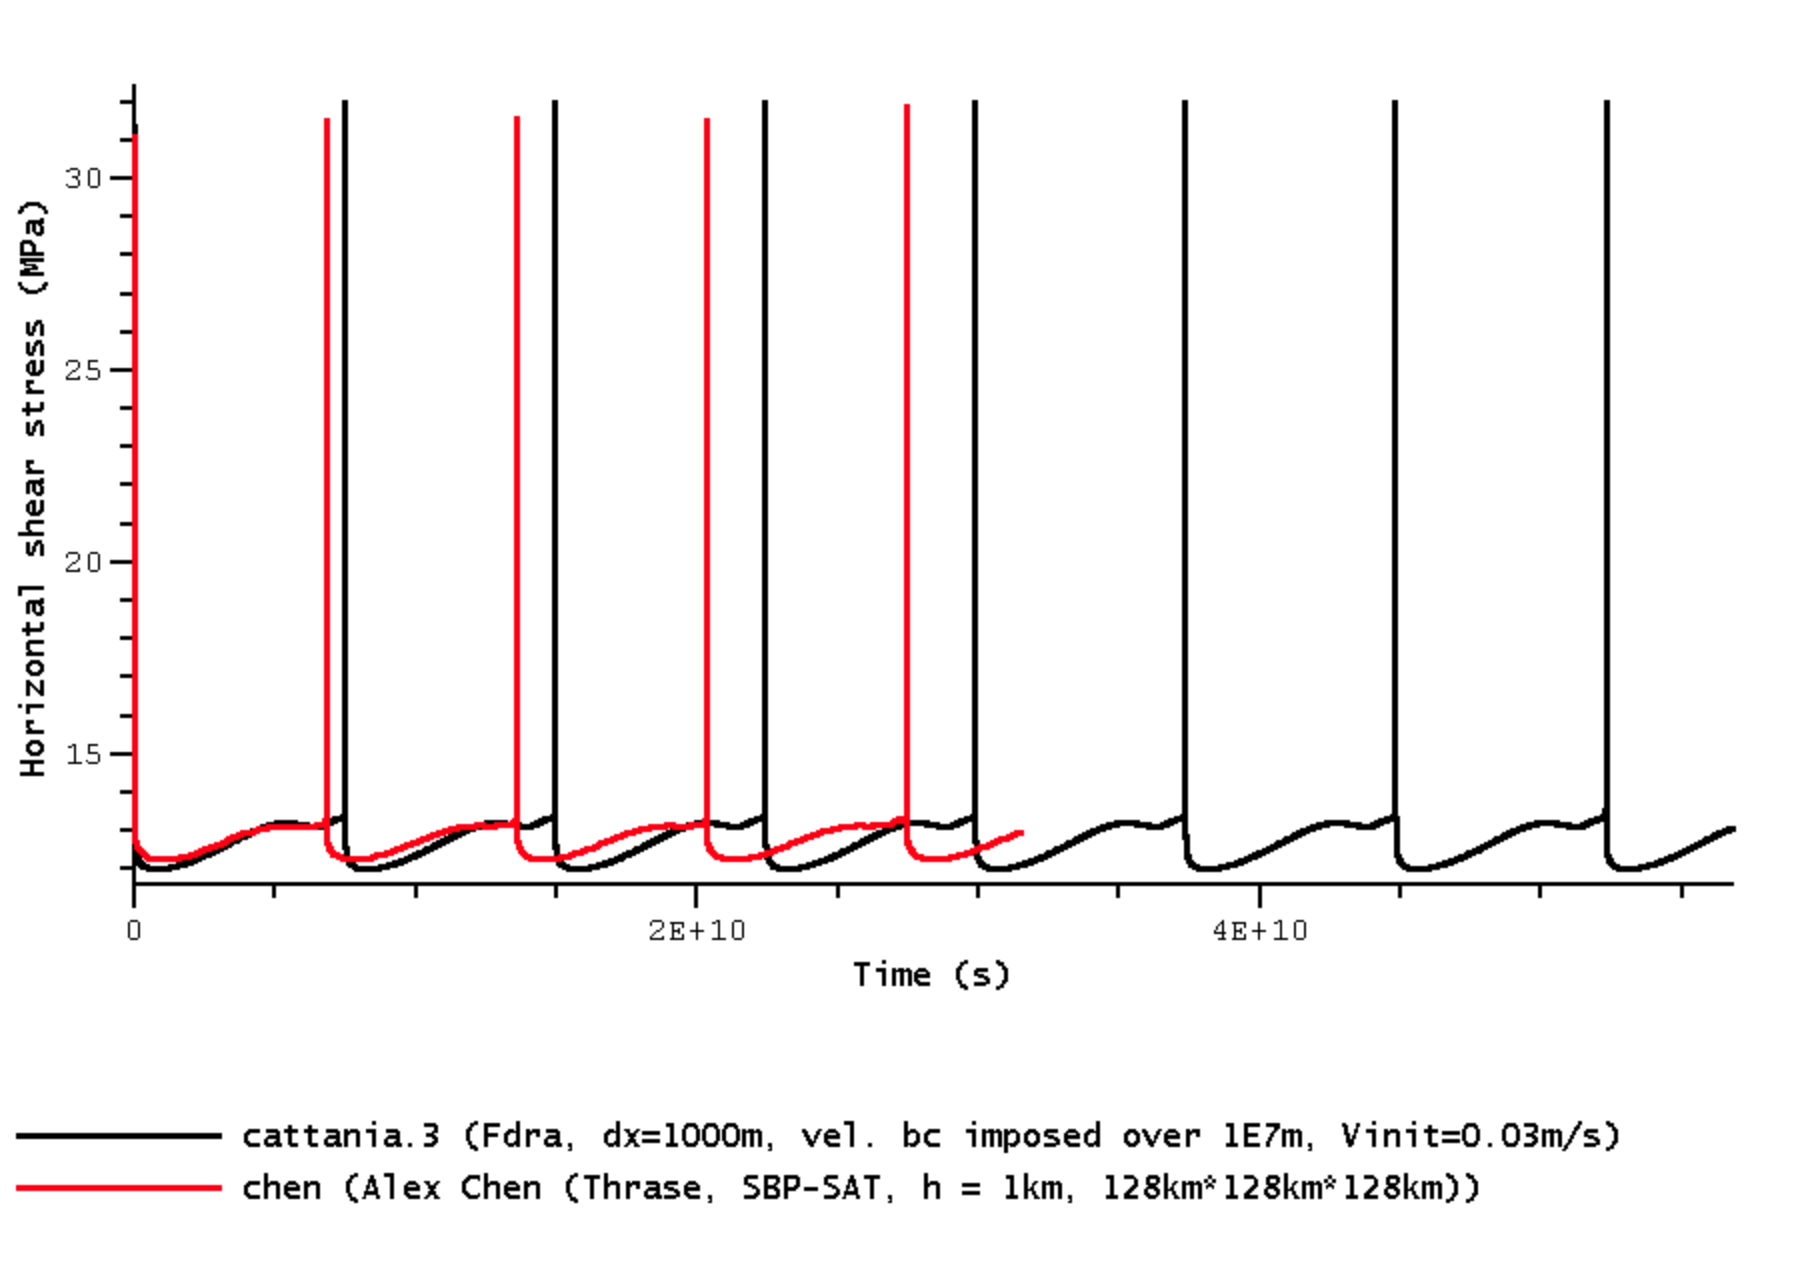
\includegraphics[width=\linewidth]{figures/sample-shearstress.png}
    \caption{Comparison of shear stress along slip directions}
    \label{fig:enter-label}
\end{figure}

We then compare the slip for the same location on the fault.

\begin{figure}
    \centering
    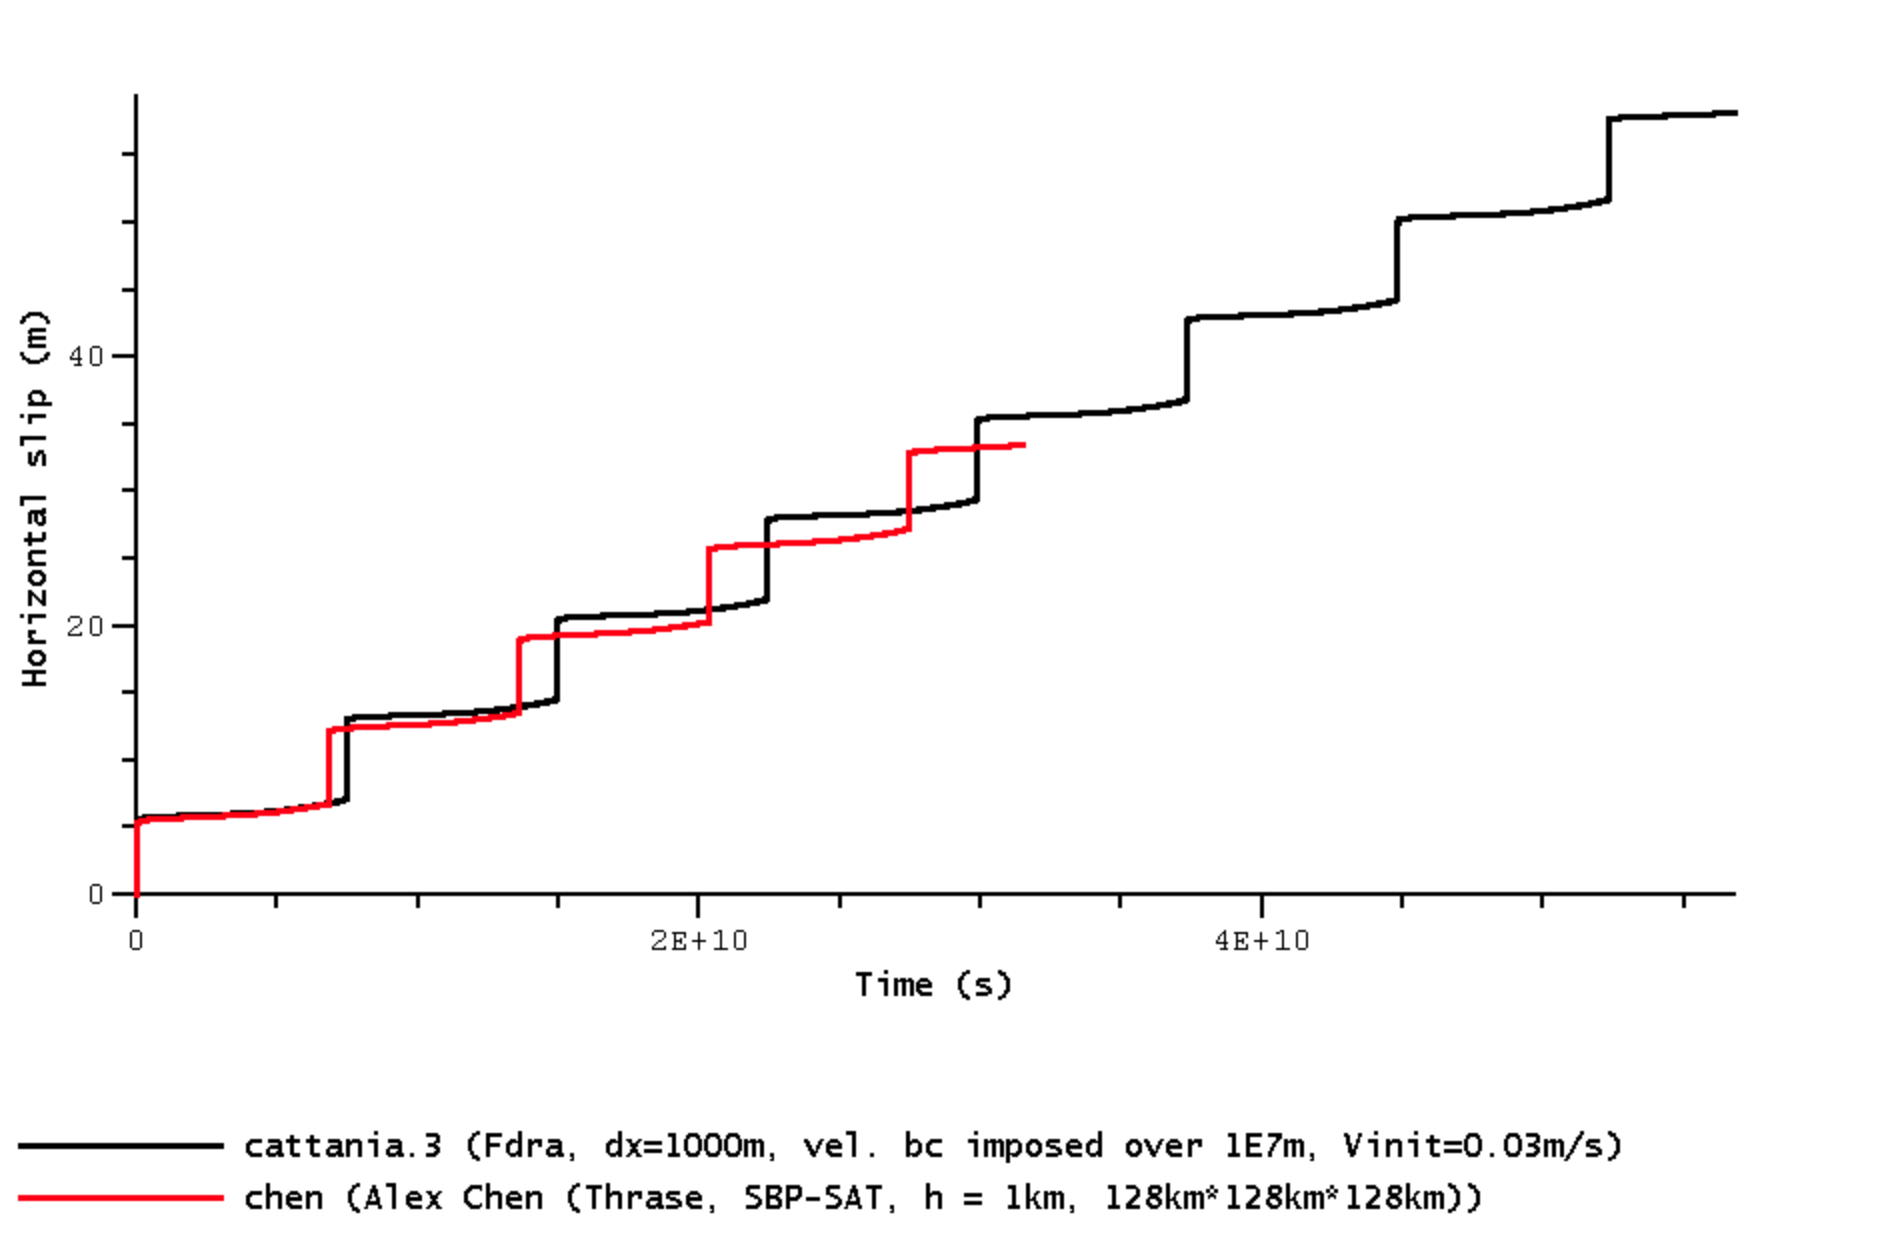
\includegraphics[width=\linewidth]{figures/sample-slip-2.png}
    \caption{Comparison of shear stress along slip directions}
    \label{fig:enter-label}
\end{figure}

Preliminary results have shown agreement in the modeling of the same problems using different methods.
Current results from other simulations are mainly based on boundary element methods, which take hours to run.
Our methods are volume-based and have more than 100 times higher degrees of freedom.
With the GPU-accelerated approach, our simulation time is cut to around ~4 hours, this is down from weeks and months of estimated time using direct methods if we have sufficient large enough memory for matrix factorization.

More results will be added to this subsection ...